\documentclass[../Main.tex]{subfiles}

\begin{document}
In this chapter, we consider a better method than that of IB Fluid Dynamics for working with large Reynolds numbers.
\section{Euler and Prandtl Limits}
Recall \eqnref{eqnNavierStokes} (Navier-Stokes equation):
\begin{equation*}
    \rho \frac{D \vec u}{D t} = \vec f = \nabla p + \mu \nabla^2 \vec u
    \tag{\ref{eqnNavierStokes}}
\end{equation*}
As an example, consider flow at speed $U$ past a body of size $L$. The nondimensionalisation with respect to $U$, $L$ and $P = \rho U^2$ is:
\begin{equation*}
    \Re \left(\St\frac{\partial u^*}{\partial t^*} + (\vec{u}^* \cdot \nabla^*) \vec{u}^*\right) = -\Re\nabla^* p^* + \nabla^{* 2} \vec{u}^*
\end{equation*}

Then, if we argue $\frac{1}{\Re} \nabla^{*2} \vec u^* \ll 1$, we get the Euler equation:
\begin{equation}
    \rho \frac{D \vec u}{D t} = \vec f - \nabla p
    \label{eqnEuler}
\end{equation}
However, this argument is dangerous! Mathematically, \eqnref{eqnNavierStokes} (Navier-Stokes equation) is second-order in space, whereas \eqnref{eqnEuler} (Euler equation) is only first-order. We need to drop the no-slip condition and can only impose no-penetration.

The Euler limit \textit{is} a good approximation sometimes: it is good for behaviour far from boundaries (such as water waves), impulsive motion (at small time scales from the impulse, where the viscosity has not had time to diffuse yet) and the lift on an aerofoil (but not the drag). The key result from IB Fluid Dynamics that indicated this is not such a good limit was that there is no drag on a translating sphere -- d'Alambert's Paradox.

The flaw in the argument is assuming that the flow has a length scale $L$ everywhere. Instead, near the rigid boundaries, we observe thin regions of the flow where there are large spatial gradients, and so $\mu \nabla^2 \vec u$ is comparable to $\rho (\vec{u} \cdot \nabla) \vec u$. These thin regions allow the no-slip boundary condition to be satisfied. See example~\ref{exStagnationPoint}, where such a thin layer was observed to be confining vorticity.

%TODO: Consider whether to include the example of flow past a rigid plate.

These thin layers are called \underline{boundary layers}. They have a width $\delta \sim \sqrt{\nu T}$ (the diffusive length), and note that:
\begin{equation*}
    \frac{\delta}{L} = \sqrt{\frac{\nu}{UL}} = \Re^{-\frac12} \ll 1
\end{equation*}
which means $\delta \ll L$, and these are thin layers (as we supposed above). Inside boundary layers, viscosity is important. Outside of the boundary layers, the Euler limit is a good approximation.

\begin{warning}
    The thin regions, despite being called boundary layers, may not always be at boundaries. For example, they may be needed for disturbances like jets of fluid.
\end{warning}

The Prandtl limit concerns the details of the flow in these thin layers and leads to the \textit{boundary layer equations}.

\begin{figure}
    \centering
    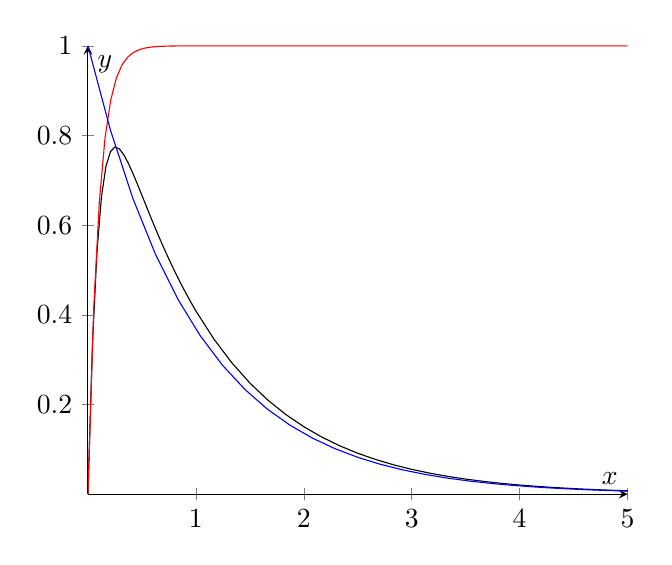
\begin{tikzpicture}[scale=1]
        \begin{axis}[
                axis lines=middle,
                xlabel={$x$},
                ylabel={$y$}
            ]
            \def\smallepsilon{0.1}
            \addplot[samples=25, domain=0:1] {(exp(-x) - exp(-x / \smallepsilon)) / (1 - \smallepsilon)};
            \addplot[samples=25, domain=1:5] {(exp(-x) - exp(-x / \smallepsilon)) / (1 - \smallepsilon)};

            \addplot[red, samples=20, domain=0:1] {1-exp(-x / \smallepsilon)};
            \addplot[red, samples=5, domain=1:5] {1-exp(-x / \smallepsilon)} node[right] {$Y(\xi)$};

            \addplot[blue, samples=25, domain=0:5] {exp(-x)};
        \end{axis}
        %TODO: Perhaps add a key? Also figure out why the blue line does not match
    \end{tikzpicture}
    \caption{Plot of toy problem}
    \label{figToyProblem}
\end{figure}

\begin{example}[Illustrative toy model]
    Consider the ODE problem:
    \begin{equation*}
        \epsilon y''(x) + y' + e^{-x}
    \end{equation*}
    with boundary conditions $y(0) = 0, y \to 0$ as $x \to \infty$. Here $0 < \epsilon \ll 1$.

    Note that this is somewhat similar to the Navier-Stokes equation in the high-$Re$ regime. We have a small constant multiplying the second derivative, and a boundary condition that is vaguely like no-slip.

    Unlike Navier-Stokes, we can solve this exactly to get:
    \begin{equation*}
        \frac{e^{-x} - e^{-\frac x \epsilon}}{1-\epsilon}
    \end{equation*}
    %TODO: plot this.
    We see that there is an layer of width $O(\epsilon$) near the origin where $y \propto x$, and far from the origin we see $y \propto \frac1x$. We will also see how to solve this with the two limiting procedures.

    In the ``Euler limit'', set $\epsilon = 0$ to get $y = e^{-x} + A$. We can only get one boundary condition to work, $y(\infty) = 0$, which requires $A = 0$. The fact that we cannot get the $y(0)$ boundary condition suggests we need a layer on which $y''$ is large.

    We work out the thickness of this boundary layer by scaling: we need $\epsilon y'' \sim y'$ for the second derivative to contribute, which means:
    \begin{equation*}
        \frac{\epsilon}{\delta^2} \sim \frac1\delta \implies \delta \sim \epsilon
    \end{equation*}

    Then to find a solution we set $\delta = \epsilon$ and work in the new coordinates $\xi = \frac x \epsilon$. The equation for $Y(\xi) = y(x)$ is:
    \begin{equation*}
        Y'' + Y' + \epsilon e^{-\xi\epsilon} = 0,\quad Y(0) = 0.
    \end{equation*}
    Then $Y(\xi) = B(1 - e^{-\xi}) + O(\epsilon)$. We fix $B$ by matching in the following way:
    \begin{equation*}
        \lim_{\xi \to \infty} Y(\xi) = \lim_{x \to 0} y(x)
    \end{equation*}
    which means $B = 1$. Then $1 - e^{-\xi}$ and $e^{-x}$ are the leading-order terms in an asymptotic expansion for the exact solution and $\epsilon \to 0$ with $\xi$ fixed, and for $\epsilon \to 0$ with $x$ fixed, respectively.
\end{example}
\section{The Boundary Layer Equations}
Consider two-dimensional flow with $\Re \gg 1$. Assume the outer inviscid fluid is known, either by the problem specification or by solving the Euler equation. In general this satisfies no-penetration but not no-slip at the boundary.

\begin{figure}
    \centering
    \begin{tikzpicture}[scale=1]
        
    \end{tikzpicture}
    \caption{Diagram of Boundary Layers}
    \label{figBoundaryLayer}
\end{figure}

Consider a setup as in figure~\ref{figBoundaryLayer}. Assume that the boundary layer thickness $\delta$ is much less than the length scale $L$ of variation in the $x$ direction (thin layer approximation). Then we can make the following scaling arguments:
\begin{enumerate}
    \item $v(0) = 0$ (no penetration) and $\frac{\partial v}{\partial y} = -\frac{\partial u}{\partial x} \sim \frac U L$ means that $v \sim \frac{\delta }{L} U \ll U$. That is, the flow is almost parallel to the boundary.
    \item Approximate $\nabla^2$ by $\frac{\partial^{2}}{\partial y^{2}}$, valid because $\delta \ll L$.
    \item In $(\vec{u} \cdot \nabla)\vec u$, we find $u \frac{\partial }{\partial x} \sim v \frac{\partial }{\partial y}$ by point 1, which both scale like $\frac U L$. If we have a time-dependent problem then $T \sim \frac L U$ and so $\frac{\partial }{\partial t} \sim \frac{U}{L}$ also. The boundary layer thickness $\delta$ is determined by a balance between advection and viscous diffusion in the momentum equation (or vorticity equation):
        \begin{align*}
            \rho (\vec{u} \cdot \nabla)u &\sim \mu \nabla^2u \\
            \rho \frac{U}{L} U \sim \mu \frac{1}{\delta^2} U \\
            \implies \delta &= \sqrt{\frac{\nu L}{U}}
        \end{align*}
    \item Outside the boundary layer, $\frac y \delta \to \infty$ and $u \to U(x, t)$. The $x$-momentum equation reduces to:
        \begin{equation*}
            \rho \left(\frac{\partial U}{\partial t} + U \frac{\partial U}{\partial x} \right) = -\frac{\partial p}{\partial x}
        \end{equation*}
        where we have removed the term $V \frac{\partial U}{\partial y}$ because it is zero to leading order (no penetration into the boundary layer). This suggests that pressure variations along the boundary layer $\Delta_x p = O(\rho U^2)$. In the boundary layer, the $y$ momentum equation gives:
        \begin{equation*}
            \rho \frac{D v}{D t} = -\frac{\partial p}{\partial y} + \mu \frac{\partial^{2}v}{\partial y^{2}}
        \end{equation*}
        and by point 3, we have chosen $\delta$ so that the advection term and diffusion terms are comparable -- they are both of order $\rho \frac U L \frac\delta L U = \rho U^2 \delta$. Therefore, the pressure variation across the boundary layer is $\Delta_y p \sim \rho U^2 \delta^2 / L^2$ which is much less than the variation $\Delta_x p$ across the boundary layer. We can therefore say that $p \approx p(x, t)$.
\end{enumerate}
In summary, in a boundary layer we have:
\begin{align}
    \rho \left(\frac{\partial u}{\partial t} + u \frac{\partial u}{\partial x} + v \frac{\partial u}{\partial y}\right) &= \rho \frac{\partial U}{\partial t} + U \frac{\partial U}{\partial x} \label{eqnBdyLayer} \\
    \frac{\partial u}{\partial x} &= \frac{\partial v}{\partial y} \nonumber
\end{align}
where \eqnref{eqnBdyLayer} is known as the \underline{boundary layer equation}. Technically, we should refer to the \textit{boundary layer equations} with the incompressibility equation included.

The boundary conditions are generally one from the problem and one matching condition. For example, for a stationary rigid body at $y = 0$,
\begin{align*}
    u = v = 0 \text{ on } y = 0& \quad\text{no slip/penetration} \\
    u \to U(x, t) \text{ as } \frac y \delta \to \infty& \quad\text{matching condition}
\end{align*}
\section{Boundary Layer on a Flat Plate}
Consider a uniform flow $U(x, t) = \text{const}$. Consider a flat, semi-infinite plate $y = 0, x > 0$. As stated, there is no length scale $L$ in the $x$ direction. Assume $L = O(1)$, so $L = x$. As with the scalings, set $\delta = \sqrt{\frac{\nu x}{U}}$.

We can work in terms of a streamfunction $\psi(x, y)$, so $u = \frac{\partial \psi}{\partial x}$ and $v = -\frac{\partial\psi}{\partial x}$. This scales as $\psi \sim U\delta(x)$, and so we try a similarity solution of the form:
\begin{equation*}
    \psi(x, y) = U \delta(x) f(\eta)
\end{equation*}
where we set $\eta = \frac{y}{\delta(x)}$. As with the gravity current, it is wise to calculate derivatives in terms of $\eta$ and $\delta$:
\begin{align*}
    \frac{\partial }{\partial x} (U\delta) = \frac12 \frac{U\delta}{x} && \frac{\partial \eta}{\partial x} = -\frac12 \frac{\eta}{x} && \frac{\partial }{\partial y} = \frac1\delta \frac{\partial }{\partial \eta}
\end{align*}
Then we can find the velocities:
\begin{align*}
    u = \frac{\partial \psi}{\partial y} = U f'(\eta) && v = -\frac{\partial \psi}{\partial x} = -\left[\frac12 \frac{U\delta}{x} f(\eta) -\frac12 U\delta \frac{\eta}{x} f'(\eta)\right]
\end{align*}
The steady boundary layer equation is:
\begin{equation*}
    u \frac{\partial u}{\partial x} + v \frac{\partial u}{\partial y} = U \frac{\partial U}{\partial x} + \nu \frac{\partial^{2}u}{\partial y^{2}}
\end{equation*}
which gives (using our similarity solution):
\begin{align*}
    \left(U f'\right)\left(-\frac12 \frac{\eta}{x}U f''\right) + \frac12 \frac{U\delta}{x} \left(\eta f' - f\right) \left(\frac{Uf''}{\delta}\right) &= \nu \frac{Uf'''}{\delta^2} \\
    -\frac12 \frac{U\delta}{x} \left(f(\eta)\right) \left(\frac{Uf''(\eta)}{\delta}\right) &= \nu \frac{Uf'''(\eta)}{\delta^2} \\
\end{align*}
and by cancelling $\delta$, we get the ODE:
\begin{equation*}
    -\frac12 f(\eta) f''(\eta) = f'''(\eta)
\end{equation*}
with boundary conditions $f(0) = f'(0) = 0$, $f'(\eta) \to 1$ as $\eta \to\infty$. This must be solved numerically and the shooting method discussed in example~\ref{exStagnationPoint} is appropriate. The numerical solution for $f'$ gets within $1\%$ of its limit $1$ by $\eta = 5$, and thereafter tends to $1$ exponentially. It also has $f \sim \eta - 1.72$ as $\eta \to \infty$, which means:
\begin{equation*}
    v = \frac12 \frac{U\delta}{x}(\eta f'(\eta) - f(\eta)) \sim 0.86 \frac{U\delta}{x} = 0.86 \sqrt{\frac{\nu U}{x}}
\end{equation*}
We note this key difference from the Euler equation: here $v$ is non-zero (but small). This is because, moving downstream, the boundary layer widens by $x^{\frac12}$ and so there is more fluid with speed less than $U$, so some must be moving upwards by mass conservation. Equivalently, the effective no-penetration boundary condition for the outer flow is at $y = \delta^* = 1.72\delta$.

We can also calculate the drag (per unit length normal to the flow direction along the plate), away from the ends,
\begin{equation*}
    \int_0^l \left(\mu \left.\frac{\partial u}{\partial y}\right|_{y = 0}\right) dx = \int_{0}^{l} \mu \frac{U}{\delta} f''(0) dx
\end{equation*}
and the numerical solution has $f''(0) = 1.72$. The drag is then:
\begin{equation*}
    2\mu U f''(0) \sqrt{\frac{U l }{\nu}} = 2f''(0) \rho U^2 l \sqrt{\frac{\nu}{Ul}}
\end{equation*}
where we note the first answer includes the viscous scaling and $\Re^{\frac12}$, and the second answer includes the inertial scaling and $\Re^{-\frac12}$.
\end{document}